\subsection{Hierarchical Structures}
\label{Section 2.2.2}

The representation of sequences in terms of lists generalizes naturally to
represent sequences whose elements may themselves be sequences.  For example,
we can regard the object

\begin{codeBlock}
>>> ((1, 2), 3, 4)
((1, 2), 3, 4)
\end{codeBlock}

\noindent
as a sequence of three items, the first of which is itself a sequence,
\code{(1, 2)}.  Indeed, the notation says so directly, which is a change from
the original: there the same object is built by \code{(cons (list 1 2) (list 3
4))} and prints as \code{((1 2) 3 4)}, and one has to know the printing rule to
see why the first list nests while the second spreads out.\footnote{Lisp prints
a pair as its \code{car}, a dot, and its \code{cdr}, but with a special case
that is almost always in force: when the \code{cdr} is itself a chain, the dot
is dropped and the printer keeps walking, so the tail's elements come out as
siblings.  \code{cons} puts \code{(1 2)} in the \code{car}, which is a single
element and therefore nests, and \code{(3 4)} in the \code{cdr}, which is the
rest-of-the-list position and is therefore walked into.  The structure is
symmetrical; only the printing is not.  Tuples have no such rule, having no
\code{cdr} to walk.} \link{Figure 2.5} shows the representation of this
structure in terms of pairs, as the original builds it.

% figure 2.5
\begin{imageFigure}{How the original represents \code{((1, 2), 3, 4)} as a
  chain of pairs.}
  % How the original represents ((1, 2), 3, 4) as a chain of pairs, for Section
% 2.2.2. Redrawn from upstream's figure 2.5 so that the three call-out labels
% use tuple notation: the shape being drawn is Scheme's, but the object being
% described is the one the surrounding text writes with commas.
%
% Coordinates are in millimetres with y running downwards, so the numbers below
% read top-to-bottom in the order the figure does. A pair is two 8mm cells side
% by side; a cell whose cdr is nil carries the conventional diagonal stroke.

\begin{tikzpicture}[
  y = -1mm, x = 1mm,
  % A pair is drawn as ONE rounded rectangle with a divider through it, not as
  % two boxes side by side: rounding two abutting boxes would round the inner
  % edges as well, which is not how the original's cells look.
  pair/.style   = {draw, rounded corners=1.2pt, fill=black!5, minimum width=16mm,
                   minimum height=7mm, inner sep=0pt, outer sep=0pt},
  % Geometry only, for anchoring pointers to each half.
  half/.style   = {minimum width=8mm, minimum height=7mm,
                   inner sep=0pt, outer sep=0pt},
  leaf/.style   = {draw, rounded corners=1pt, fill=white, minimum width=8mm,
                   minimum height=7mm, inner sep=0pt, outer sep=0pt,
                   font=\ttfamily\footnotesize},
  dot/.style    = {circle, fill, inner sep=1.1pt},
  arrow/.style  = {-{Latex[length=1.6mm, width=1.4mm]}, thin},
  label/.style  = {font=\ttfamily\scriptsize, inner sep=1pt},
]

% --- the pairs: each is a left (car) and right (cdr) cell ---
\foreach \n/\x/\y in {pA/22/0, pC/62/0, pD/82/0, pB/22/15, pBb/44/15} {
  \node[half] (\n l) at (\x, \y) {};
  \node[half] (\n r) at (\x+8, \y) {};
  \node[pair] (\n)   at (\x+4, \y) {};
  \draw (\n l.north east) -- (\n l.south east);
  \node[dot]  (\n d) at (\x, \y) {};
}
% cdr pointers, except where the cdr is nil
\foreach \n in {pA, pC, pB} \node[dot] (\n rd) at ($(\n r.center)$) {};

% --- nil: the conventional diagonal through the final cdr ---
\draw (pDr.south west) -- (pDr.north east);
\draw (pBbr.south west) -- (pBbr.north east);

% --- leaves ---
\node[leaf] (l1) at (22, 30) {1};
\node[leaf] (l2) at (44, 30) {2};
\node[leaf] (l3) at (62, 15) {3};
\node[leaf] (l4) at (82, 15) {4};

% --- pointers ---
\draw[arrow] (pAd)  -- (pBl.north);      % car of the whole structure is (1, 2)
\draw[arrow] (pArd) -- (pCl.west);       % cdr runs on to 3
\draw[arrow] (pBd)  -- (l1.north);
\draw[arrow] (pBrd) -- (pBbl.west);
\draw[arrow] (pBbd) -- (l2.north);
\draw[arrow] (pCd)  -- (l3.north);
\draw[arrow] (pCrd) -- (pDl.west);
\draw[arrow] (pDd)  -- (l4.north);

% --- call-out labels, in the notation the section is written in ---
\node[label] (topA) at (22, -11) {((1, 2), 3, 4)};
\draw[arrow] (topA.south) -- (pAl.north);
\node[label] (topC) at (62, -11) {(3, 4)};
\draw[arrow] (topC.south) -- (pCl.north);
\node[label] (leftB) at (4, 15) {(1, 2)};
\draw[arrow] (leftB.east) -- (pBl.west);

\end{tikzpicture}

\end{imageFigure}

Another way to think of sequences whose elements are sequences is as
\newterm{trees}.  The elements of the sequence are the branches of the tree,
and elements that are themselves sequences are subtrees.  \link{Figure 2.6}
shows the same structure viewed as a tree.

% figure 2.6
\begin{imageFigure}{The structure in \link{Figure 2.5} viewed as a tree.}
  % The structure ((1, 2), 3, 4) viewed as a tree, for Section 2.2.2.
%
% Upstream's figure labels the root and the one interior node with Lisp's
% printed form. Ours uses the tuple notation the section is written in, which
% is the whole reason this figure is redrawn rather than inherited: the shape
% of the tree is the same in both languages, but the labels are not.
%
% Leaves are spaced evenly and every parent sits at the midpoint of its
% children, matching the layout of the other tree figures in the book.

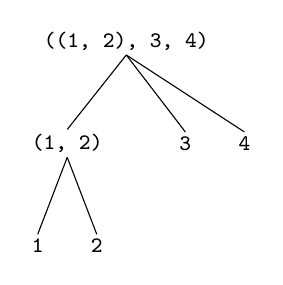
\begin{tikzpicture}[
  x = 15mm, y = -13mm,
  every node/.style = {font=\ttfamily\footnotesize, inner sep=1.5pt},
  edge/.style = {draw, thin},
]

\node (root) at (1.0, 0) {((1, 2), 3, 4)};
\node (sub)  at (0.5, 1) {(1, 2)};
\node (n3)   at (1.5, 1) {3};
\node (n4)   at (2.0, 1) {4};
\node (n1)   at (0.25, 2) {1};
\node (n2)   at (0.75, 2) {2};

% Anchored at the base of the parent rather than its border: the root's label
% is wide enough that border-to-border edges would leave from under the middle
% of the text instead of from the node.
\foreach \parent/\child in {root/sub, root/n3, root/n4, sub/n1, sub/n2}
  \draw[edge] (\parent.south) -- (\child.north);

\end{tikzpicture}

\end{imageFigure}

Recursion is a natural tool for dealing with tree structures, since we can
often reduce operations on trees to operations on their branches, which reduce
in turn to operations on the branches of the branches, and so on, until we
reach the leaves of the tree.  As an example, compare the \code{length}
procedure of \link{Section 2.2.1} with the \code{count\_leaves} procedure,
which returns the total number of leaves of a tree:

\begin{codeBlock}
>>> x = ((1, 2), 3, 4)
>>> len(x)
3
>>> count_leaves(x)
4
>>> (x, x)
(((1, 2), 3, 4), ((1, 2), 3, 4))
>>> len((x, x))
2
>>> count_leaves((x, x))
8
\end{codeBlock}

\noindent
To implement \code{count\_leaves}, recall the recursive plan for computing
\code{length}:

\begin{itemize}
\item
\code{length} of a sequence \code{x} is 1 plus \code{length} of the rest of
\code{x}.

\item
\code{length} of the empty sequence is 0.
\end{itemize}

\noindent
\code{count\_leaves} is similar.  The value for the empty sequence is the same:

\begin{itemize}
\item
\code{count\_leaves} of the empty sequence is 0.
\end{itemize}

\noindent
But in the reduction step, where we strip off the first element, we must take
into account that it may itself be a tree whose leaves we need to count.  Thus,
the appropriate reduction step is

\begin{itemize}
\item
\code{count\_leaves} of a tree \code{x} is \code{count\_leaves} of the first
element of \code{x} plus \code{count\_leaves} of the rest of \code{x}.
\end{itemize}

\noindent
Finally, by taking first elements we reach actual leaves, so we need another
base case:

\begin{itemize}
\item
\code{count\_leaves} of a leaf is 1.
\end{itemize}

\noindent
To aid in writing recursive procedures on trees, Scheme provides the primitive
predicate \code{pair?}, which tests whether its argument is a pair.  We can
define it:

\begin{codeBlock}
>>> def is_pair(x):
...     return isinstance(x, tuple)
\end{codeBlock}

\noindent
\code{isinstance} asks whether a value is of a given type, and here the
question is whether we have reached a leaf or are still looking at a branch.
Note that the length does not enter into it.\footnote{Which makes the inherited
name a little awkward.  In \link{Section 2.1} a pair was a tuple of exactly two
elements; \code{is\_pair} here is true of a tuple of any length, because that
is what the original's \code{pair?} asks.  A Scheme list of three elements
\emph{is} a pair---its \code{car} is the first element and its \code{cdr} is
the other two---so \code{pair?} has never meant ``has two elements.''  It means
``is compound rather than atomic,'' and \code{isinstance(x, tuple)} is exactly
that question for us.  Defining it as \code{len(x) == 2} would report
\code{((1, 2), 3, 4)} to be a leaf, and \code{count\_leaves} would answer 1.}

Here is the complete procedure:

\begin{codeBlock}
>>> def count_leaves(x):
...     if x == ():
...         return 0
...     elif not is_pair(x):
...         return 1
...     else:
...         return count_leaves(x[0]) + count_leaves(x[1:])
\end{codeBlock}

\noindent
Note that we test the empty tuple with \code{x == ()} and not with \code{not
x}, which is how we asked the same question in \link{Section 2.2.1}.  The
difference did not matter there and matters here.  In \link{Section 2.2.1} the
argument was always a sequence, and the only false sequence is the empty one.
A tree is another matter: the recursion descends onto the leaves as well as the
branches, and a leaf may be any object at all---including \code{0}, which is
false.  Written \code{not x}, the procedure would take a leaf of \code{0} for
the end of a branch and stop counting, so that \code{count\_leaves((0, 1))}
answered 1 where it should answer 2.\footnote{This is among the more common
ways to be caught out by Python's rule that an empty container and a zero are
alike false.  The rule is convenient exactly as long as the only falsehood one
expects is emptiness, and a tree of numbers is the ordinary case where that
stops being so.}

The original adds a footnote here warning that the order of its first two
clauses matters, since the empty list satisfies \code{null?} and is also not a
pair, so that testing for a leaf first would count the empty list as a leaf.
For us the order does not matter, and the reason is the single point on which
our \code{is\_pair} disagrees with \code{pair?}: an empty tuple is still a
tuple, so \code{is\_pair(())} is true where \code{(pair? '())} is false, and an
empty branch cannot be taken for a leaf however the clauses are arranged.  What
we may not do is leave the clause out altogether; without it the procedure asks
a tuple of no elements for its first, and gets an \code{IndexError}.

\begin{exerciseGroup}
\phantomsection\label{Exercise 2.24}
\exerciseHeading{Exercise 2.24:} Suppose we evaluate the
expression \code{(1, (2, (3, 4)))}.  Give the result printed by the
interpreter, the corresponding box-and-pointer structure as the original would
build it, and the interpretation of this as a tree (as in \link{Figure 2.6}).

\phantomsection\label{Exercise 2.25}
\exerciseHeading{Exercise 2.25:} Give combinations of \code{[0]}
and \code{[1:]} that will pick 7 from each of the following sequences:

\begin{codeBlock}
(1, 3, (5, 7), 9)
((7,),)
(1, (2, (3, (4, (5, (6, 7))))))
\end{codeBlock}

In the original this exercise is a genuine puzzle, because \code{car} and
\code{cdr} are the only two things one can do to a pair and the answer must be
spelled as a composition of them---\code{(cadr (car (cdr (cdr x))))} for the
first.  Here it is less of one, since Python can index straight to a position
and the answer to the first is \code{x[2][1]}.  Give both: first the
composition of \code{[0]} and \code{[1:]}, which is the exercise the original
is setting, and then the shortest indexing that gets there.  The point of doing
it twice is to see that the second is the first with the steps collapsed---the
brackets are not a different mechanism, only a briefer notation for the same
descent.

\phantomsection\label{Exercise 2.26}
\exerciseHeading{Exercise 2.26:} Suppose we define \code{x} and
\code{y} to be two sequences:

\begin{codeBlock}
>>> x = (1, 2, 3)
>>> y = (4, 5, 6)
\end{codeBlock}

The original asks what three of its procedures print when applied to these.
Recall what each does.  \code{append} runs two lists together into one, so that
the elements of the second follow the elements of the first.  \code{cons} adds
a single item to the front of a list, and here that item is itself a list.
\code{list} makes a new list of the things given to it, which here are two
lists, so the result has two elements.

\begin{codeBlock}
(append x y)
(cons x y)
(list x y)
\end{codeBlock}

Work out what each prints.  Then write, for each, the expression that produces
the same result from our tuples \code{x} and \code{y}, and say which of the
three Python spells most differently from the original and why.

\phantomsection\label{Exercise 2.27}
\exerciseHeading{Exercise 2.27:} Modify your \code{reverse}
procedure of \link{Exercise 2.18} to produce a \code{deep\_reverse} procedure
that takes a sequence as argument and returns as its value the sequence with
its elements reversed and with all subsequences deep-reversed as well.  For
example,

\begin{codeBlock}
>>> x = ((1, 2), (3, 4))
>>> x
((1, 2), (3, 4))
>>> reverse(x)
((3, 4), (1, 2))
>>> deep_reverse(x)
((4, 3), (2, 1))
\end{codeBlock}

\phantomsection\label{Exercise 2.28}
\exerciseHeading{Exercise 2.28:} Write a procedure \code{fringe}
that takes as argument a tree (represented as a sequence) and returns a
sequence whose elements are all the leaves of the tree arranged in
left-to-right order.  For example,

\begin{codeBlock}
>>> x = ((1, 2), (3, 4))
>>> fringe(x)
(1, 2, 3, 4)
>>> fringe((x, x))
(1, 2, 3, 4, 1, 2, 3, 4)
\end{codeBlock}

\phantomsection\label{Exercise 2.29}
\exerciseHeading{Exercise 2.29:} A binary mobile consists of two
branches, a left branch and a right branch.  Each branch is a rod of a certain
length, from which hangs either a weight or another binary mobile.  We can
represent a binary mobile using compound data by constructing it from two
branches:

\begin{codeBlock}
>>> def make_mobile(left, right):
...     return (left, right)
\end{codeBlock}

A branch is constructed from a \code{length} (which must be a number) together
with a \code{structure}, which may be either a number (representing a simple
weight) or another mobile:

\begin{codeBlock}
>>> def make_branch(length, structure):
...     return (length, structure)
\end{codeBlock}

\begin{enumerate}[a.]

\item
Write the corresponding selectors.  \code{left\_branch} and
\code{right\_branch} return the branches of a mobile; \code{branch\_length} and
\code{branch\_structure} return the components of a branch.

\item
Using your selectors, define a procedure \code{total\_weight} that returns the
total weight of a mobile.

\item
A mobile is said to be \newterm{balanced} if the torque applied by its top-left
branch is equal to that applied by its top-right branch (that is, if the length
of the left rod multiplied by the weight hanging from that rod is equal to the
corresponding product for the right side) and if each of the submobiles hanging
off its branches is balanced.  Design a predicate \code{is\_balanced} that
tests whether a binary mobile is balanced.

\item
Suppose we change the representation of mobiles so that the constructors are

\begin{codeBlock}
>>> def make_mobile(left, right):
...     return (left, right)

>>> def make_branch(length, structure):
...     return (length, structure)
\end{codeBlock}

How much do you need to change your programs to convert to the new
representation?\footnote{The original changes \code{list} to \code{cons} here,
which in Scheme is a real change of representation: \code{(list a b)} is a
chain of two pairs and \code{(cons a b)} is a single pair, so the selectors
must change with it.  For us both spellings are the same two-element tuple, and
the exercise loses its teeth.  Answer the question the original is asking
instead: what would have to change if a mobile were represented some other
way---say with the two branches in the opposite order---and how much of your
code would you have to look at to find out?}

\end{enumerate}
\end{exerciseGroup}

\subsubsection*{Mapping over trees}

Just as \code{map} is a powerful abstraction for dealing with sequences,
\code{map} together with recursion is a powerful abstraction for dealing with
trees.  For instance, the \code{scale\_tree} procedure, analogous to
\code{scale\_list} of \link{Section 2.2.1}, takes as arguments a numeric factor
and a tree whose leaves are numbers.  It returns a tree of the same shape,
where each number is multiplied by the factor.  The recursive plan for
\code{scale\_tree} is similar to the one for \code{count\_leaves}:

\begin{codeBlock}
>>> def scale_tree(tree, factor):
...     if tree == ():
...         return ()
...     elif not is_pair(tree):
...         return tree * factor
...     else:
...         return ((scale_tree(tree[0], factor),)
...                 + scale_tree(tree[1:], factor))

>>> scale_tree((1, (2, (3, 4), 5), (6, 7)), 10)
(10, (20, (30, 40), 50), (60, 70))
\end{codeBlock}

\noindent
Another way to implement \code{scale\_tree} is to regard the tree as a sequence
of sub-trees and use \code{map}.  We map over the sequence, scaling each
sub-tree in turn, and return the sequence of results.  In the base case, where
the tree is a leaf, we simply multiply by the factor:

\begin{codeBlock}
>>> def scale_tree(tree, factor):
...     return tuple(map(
...         lambda sub_tree: (scale_tree(sub_tree, factor)
...                           if is_pair(sub_tree)
...                           else sub_tree * factor),
...         tree))
\end{codeBlock}

\noindent
Note that the empty case has gone.  The original still needs \code{null?} in
its first version because it walks the list pair by pair and must recognise the
end; this version hands the whole sequence to \code{map} and never sees the end
as a separate thing, since mapping over an empty sequence gives an empty
sequence without being told.

\noindent
Many tree operations can be implemented by similar combinations of sequence
operations and recursion.

\begin{exerciseGroup}
\phantomsection\label{Exercise 2.30}
\exerciseHeading{Exercise 2.30:} Define a procedure
\code{square\_tree} analogous to the \code{square\_list} procedure of
\link{Exercise 2.21}.  That is, \code{square\_tree} should behave as follows:

\begin{codeBlock}
>>> square_tree((1, (2, (3, 4), 5), (6, 7)))
(1, (4, (9, 16), 25), (36, 49))
\end{codeBlock}

Define \code{square\_tree} both directly (that is, without using any
higher-order procedures) and also by using \code{map} and recursion.

\phantomsection\label{Exercise 2.31}
\exerciseHeading{Exercise 2.31:} Abstract your answer to
\link{Exercise 2.30} to produce a procedure \code{tree\_map} with the property
that \code{square\_tree} could be defined as

\begin{codeBlock}
>>> def square_tree(tree):
...     return tree_map(square, tree)
\end{codeBlock}

\phantomsection\label{Exercise 2.32}
\exerciseHeading{Exercise 2.32:} We can represent a set as a
sequence of distinct elements, and we can represent the set of all subsets of
the set as a sequence of sequences.  For example, if the set is \code{(1, 2,
3)}, then the set of all subsets is

\begin{codeBlock}
>>> subsets((1, 2, 3))
((), (3,), (2,), (2, 3), (1,), (1, 3), (1, 2), (1, 2, 3))
\end{codeBlock}

Complete the following definition of a procedure that generates the set of
subsets of a set and give a clear explanation of why it works:

\begin{syntaxForm}
def subsets(s):
    if s == ():
        return ((),)
    else:
        rest = subsets(s[1:])
        return rest + tuple(\meta{??} for r in rest)
\end{syntaxForm}
\end{exerciseGroup}

